\documentclass[a4paper,oneside]{Tptesi2}

\usepackage[italian]{babel}
\usepackage{listings}
\usepackage{amsmath,amssymb}
\usepackage{verbatim}
\usepackage{indentfirst}
\usepackage[utf8]{inputenc}
\usepackage{subfigure}
\usepackage{algorithmic}
\usepackage{framed}
\usepackage{rotating}
\usepackage{cite}

% Packages -----------------------------------------------------------------------
%\usepackage{amsthm}
%\usepackage{amsmath}          % Non necessario se usi TPTESI2 perche' gia` incluso
%\usepackage[dvips]{graphicx}  % Non necessario se usi TPTESI2 perche' gia` incluso
%\usepackage{url} %non usare se si usa hyperref


\newcommand{\mr}{\emph{motore di ricerca}}
\newcommand{\Mr}{\emph{Motore di ricerca}}
\newcommand{\ws}{Web~service }


% Use a small font for the verbatim environment
\makeatletter  % makes '@' an ordinary character
\renewcommand{\verbatim@font}{%
  \ttfamily\footnotesize\catcode`\<=\active\catcode`\>=\active%
}
\makeatother   % makes '@' a special symbol again
%
% Simboli Matematici -------------------------------------------------------------
%\newcommand{\h}{\mathcal{H}_\infty} % scorciatoia per sequenza usata spesso
% Definizioni & Teoremi ----------------------------------------------------------
\newtheorem{teorema}{Teorema}[chapter]
\newtheorem{corollario}[teorema]{Corollario}
\newtheorem{lemma}[teorema]{Lemma}
%\theoremstyle{definition}
\newtheorem{definizione}{Definizione}[chapter]
\newtheorem{proposizione}[definizione]{Proposizione}
% Formattazione Figure -----------------------------------------------------------
\setcounter{topnumber}{3}
\setcounter{totalnumber}{3}
\def\topfraction{1}
\def\textfraction{0}
% Fuzz ---------------------------------------------------------------------------
%\hfuzz10cm %Non scassare linee che escono dal bordo
% Frontespizio -------------------------------------------------------------------
       \title{insert title\ldots}
       \author{insert candidate\ldots}
       \titolocorso{Ingegneria Informatica}
       \chair{Prof. ... \\ }
       \numberofmembers{1} %numero dei relatori
       \degreeyear{insert degree year\ldots}
       \numerocorrelatori{2} %numero dei correlatori
       \correlatori{insert correlators\ldots} % i correlatori separati da \\

%
% ---- Inclusioni (vedi piu` sotto per il comando "include" --------------
%\includeonly {introduzione,chapter1, chapter2}
%\includeonly {chapter1, chapter2, chapter3, chapter4, chapter5, chapter6}
%\includeonly{chapter6}
%
\hypersetup{%
%  pdfpagemode=FullScreen,%
  plainpages=false,%
  breaklinks,%
  pdftitle={},%
  pdfauthor={},%
  pdfsubject={},%
  pdfkeywords={},%
  colorlinks=false}

\begin{document}

\frontmatter

%\hyphenation{}
%
\pagestyle{headings} % rende attive le impostazioni sulla testata!
%
\maketitle % crea il frontespizio (ricordati di copiare "stemma.eps" nella tua directory)
%
%
%\pagenumbering{roman}
\tableofcontents % inserisce indice generale
\cleardoublepage
%\addcontentsline{toc}{chapter}{Elenco delle figure}
%\listoffigures   % inserisce indice figure
%\addcontentsline{toc}{chapter}{Elenco delle tabelle}
%\listoftables    % inserisce indice tabelle
%\addcontentsline{toc}{chapter}{Elenco degli algoritmi}
%\listofalgorithms
%
%--------------- Inizio del testo vero e proprio
%

%\cleardoublepage
%\pagenumbering{arabic}
%\input{files/ringraziamenti}
\frontmatter
\chapter{Introduzione}\label{ch:introduzione}
\ldots
\cite{gruntzig1978transluminal}

\mainmatter
\chapter{Scopo del progetto}\label{ch:scopo}

Lo scopo del progetto, dunque, è stato quindi quello di sviluppare un'applicativo nativo cross-platform che permettesse all'utente di avere una sorta di stilista digitale sempre a portata di mano. Quest'ultimo potrà infatti andare a creare il proprio armadio virtuale andando a scattare delle foto ai suoi capi di abbigliamento e, una volta aggiunti, ricercarli attraverso dei filtri.

Per quanto riguarda l'aggiunta del capo, oltre a dover inserire i dati principali del prodotto come colore, categoria e stagione, qui sotto spiegati, all'utente verrà inoltre richiesto di scattare una foto. Abbiamo pensato che l'utilizzo di un segmentatore potesse essere perfettamente votato alla causa: in questo modo l'indumento verrà completamente ritagliato dallo sfondo in modo tale da escludere eventuali altri oggetti, che oltre ad essere inutili da un punto di vista informativo potrebbero condurre in errore le reti neurali, le quali potrebbero considerarli in una eventuale raccomandazione.

I filtri che permettono di discriminare la ricerca in base a 3 diversi tag:
\begin{itemize}
\item Colore: quindi si va a filtrare tutti quegli abiti con il colore selezionato
\item Categoria: ovvero se l'indumento è un top o un bottom, ad esempio una TShirt è un top mentre un paio di jeans è un bottom.
\item Stagione: in base a quale stagione sarà più consono indossare il vestito selezionato.
\end{itemize}

Una volta aggiunti, i vestiti potranno dunque essere selezionati e l'applicazione andrà a proporre degli outfit che costituiscono un match , chiaramente in base alla correttezza di abbinamento dei colori. L'utente tuttavia avrà la facoltà, in questo caso, di poter ulteriormente filtrare i risultati in base al colore dell'indumento proposto, ed in base al mood in cui si trova e all'evento sociale per il quale utilizzerà tale outfit.

Chiaramente la raccomandazione in base a stile ed evento è adempiuta dalle due reti neurali che avevamo a disposizione: queste prenderanno inizialmente in ingresso l'indumento iniziale e proporranno una serie di abbinamenti coerenti. Ogni abbinamento verrà quindi scansionato per determinare il mood e l'evento appropriati, informazione che quindi verrà attaccata all'outfit stesso. A questo punto, una volta che l'utente deciderà di discriminare i risultati in base a questi filtri, basterà semplicemente controllare se il metadato corrispondente è coerente o meno con la cernita effettuata.

Una volta trovato l'abbinamento o gli abbinamenti l'utente dovrà essere in grado di salvarli in locale e poterli visualizzare con persistenza su un'altra tab, in modo da poter sfruttarli in più occasioni, anche qui potendo discernere in base allo stile e alla situazione sociale in cui sarebbe perfetto indossarli. Ovviamente dovrà essere in grado anche di visualizzare il mood e l'evento per cui erano stati pensati tali outfit, e inoltre dovrà poterli modificare e/o eliminarli.  

\chapter{Teoria di Kobayashi}\label{ch:teoria}

Parliamo di bias ogni qualvolta una suggesione ci porta ad agire in modo diverso da quanto saremmo soliti fare se quella particolare inclinazione non ci avesse mai colpiti. A livello psicologico, è intuibile pensare che le emozioni che proviamo potrebbero essere proprio quella influenza che ci porta a comportarci in un modo o nell'altro. Per deduzione, anche il nostro modo di vestire quotidiano e i colori indossati potrebbero far parte di quelle azioni che le varie suggestioni emotive ci portano a compiere.

Difatti per quanto riguarda la teoria filosofico-scientifica che fa da fondamento alla rete neurale che abbiamo utilizzato per suggerire l'outfit in base al mood in questo progetto è derivante dagli studi sul colore e dei suoi accostamenti dello studioso giapponese Shigenobu Kobayashi. Nel libro "Color Image Scale" edito nel 1990 oltre a studiare le possibili correlazioni con vastissimi ambiti come forme e cucina, Kobayashi si sofferma sul tema forse più filosofico,che riprende maggiormente le correnti di pensiero del Sol Levante, la sua madre patria : le emozioni.

Nel senso più letterale del termine Kobayashi associa a dei gruppi di colore una particolare emozione, dopo aver chiaramente analizzato il problema da un punto di vista psico-sociologico. Applicando i suoi studi alla moda, è intuitivo pensare che se una persona si veste usando colori prettamente scuri e cupi potrebbe esprimere una sensazione negativa mentre colori sgargianti  e luminosi potrebbero trasmettere benestare. Di fatto lo studioso giapponese va a formalizzare queste intuizioni creando così un sistema biunivoco che correla una particolare emozione ad una combinazione di colori.

Come spiegheremo più avanti, nella sezione dedicata ai modelli usati per la categorizzazione, le triplette di colore identificate da Kobayashi vengono fatte coincidere con precisi stili che riflettono l'attitudine di una persona in modo da suggerire un abbinamento corretto per ogni occasione

\chapter{Concetto di Cross Platform}\label{ch:crossplatform}

L'avanzare tecnologico e l'impronta sempre più grande che gli smartphone, o comunque i dispositivi tecnologici personali con cui interagiamo, hanno sulla nostra vita, ha reso lo sviluppo di applicativi un materia sempre più importante e remunerativa a livello globale, andando ad incidere su una fetta di mercato che riguarda quasi totalmente la popolazione mondiale.

L'approccio mobile-first la fa da padrone, in quanto ormai i computer sono stati perlopiù sostituiti da dispositivi che possiamo tenere sempre più a portata di mano come smartphones e smartwatches, e le aziende hanno sentito la necessità di spostare i loro canali di comunicazione favorendo lo sviluppo di app mobili in modo da rivolgersi ad un pubblico più vasto. E per la dura legge dell'economia si preferisce sempre pagare di meno per un progetto che è più facile da mantenere e più compatibile.
Con il concetto di cross-platform si intende infatti la capacità di sviluppare un'applicativo compilabile su diversi processori e sistemi operativi attraverso l'utilizzo di un singolo linguaggio, senza quindi creare due versioni logicamente equivalenti ma che hanno bisogno di essere scritte in linguaggi diversi per funzionare su dispositivi eterogenei.

Alcuni esempi di linguaggi cross-platform sono il C, Java, PHP, Python, ecc.. Questi infatti possono essere compilati su diverse macchine indipendentemente se su queste è stato installato un qualsiasi sistema operativo, rendendo quindi possibile scrivere codice che sarà chiaramente compatibile e condivisibile tra diversi utenti possessori di macchine diverse.

Il cross-platform è una tematica molto importante per quanto riguarda lo sviluppo di applicativi in quanto permette un risparmio di tempo considerevole in quanto non è necessario scrivere la stessa logica in linguaggi diversi, e di conseguenza anche un risparmio economico per le aziende, dovendo mantenere una singola versione di codice e non due sostanzialmente uguali come avverrebbe normalmente.

Sebbene non sia tutto oro quel che luccica in quanto uno sviluppo nativo garantisce comunque la massima espressività logica pelìr il dispositivo per cui stiamo sviluppando ed un supporto completo, la possibilità di avere un solo linguaggio per diverse piattaforme e essere capaci di creare UI identiche tra una piattaforma all'altra rende lo sviluppo cross-platform molto appetibile.

Nel nostro caso l'utilizzo di tecnologie cross-platform ci ha permesso di sviluppare una applicazione che ha la facoltà di essere compilata ed eseguita sia su device basati su Android sia IOS, nonchè possa essere convertita anche in una web app.In particolare abbiamo raggiunto il nostro scopo attraverso l'uso del framework open source Ionic e integrando Capacitor, runtime che supporta sia Swift per IOS, sia Java per Android. 

La nostra volontà è stata quella di adattare un approccio cross platform in modo tale da poter integrare la nostra web app su dispositivi mobile senza la necessità di dover implementare due diverse versioni di codice e senza il bisogno di imparare due differenti linguaggi per lo sviluppo nativo. Il risultato quindi è stato quello di una app che si modella perfettamente sia in ambiente mobile che desktop e che richiede un bassissimo livello di mantenimento, in quanto le future modifiche verranno eseguite solo su una versione di codice.


\chapter{Front End}\label{ch:frontend}

In questa sezione l'intento è quello di esporre tutte le tecnologie più importanti che sono state necessarie per sviluppare il front end della nostra applicazione. In particolare il front end si occupa di definire una interfaccia utente intuitiva attraverso la quale l'utente può interagire per inviare dati al server e assue la responsabilità di elaborare e gestire tali dati in ingresso affinchè siano conformi a quelli richiesti dal back end.

\section{Ionic}

Ionic è un framework open source creato allo scopo di realizzare app cross platform native e web app semplice, veloce ed efficiente. Rilasciato nel corso del 2013 da Drifty co. , inizialmente si basava solamente su Angular JS; tuttavia lo sviluppo è proseguito andando ad inglobare i nuovi framework per UI React, Angular e Vue.Si tratta di un modulo npm e quindi necessita di Node.js per funzionare.
In particolare questa tecnologia provvede gli strumenti per sviluppare web app e app mobile ibride basate su tecniche e pratiche moderne, integrando tecnologie web come CSS, SCSS  e HTML e per rilasciarle sul mercato mobile attraverso Capacitor o Cordova, che si occupano della conversione dell'app in modo che sia compatibile con il device in uso.
In particolare nel corso dello sviluppo abbiamo utilizzato i seguenti componenti Ionic per la realizzazione del nostro applicativo:
\begin{itemize}
\item ion-slides: è un container multisezione, dove si può  scorrere ogni sezione per visualizzare delle ion-slide. L'abbiamo utilizzata in "garment-detail" al fine di potere proporre una moltitudine di abbinamenti per il capo scelto dall'utente e in modo che quest'ultimo possa scorrere tra esse e scegliere quella che è più di suo gusto.
\item ion-content: provvede un area per i contenuti ed offre diversi metodi per controllare lo scrolling. Viene utilizzato una singola volta in tutti i nostri componenti al fine di poter definirne i contenuti.
\item ion-header: è il componente che definisce la parte estrema superiore dell'app. Permette la definizione al suo interno di una toolbar e la contestualizzazione della tab o pagina in cui siamo attraverso la possibilità di aggiungergli un testo.
\item ion-img: è il tag sostitutivo al quasi omonimo tag <img> di HTML. In realtà  per quanto lo scopo possa essere similare, le caratteristiche e le funzioni della versione Ionic sono nettamente superiori. In particolare nel nostro caso, dovendo visualizzare potenzialmente molte foto (chiaramente va in base alla dimensione dell'armadio dell'utente), questo componente ci è estremamente utile in quanto implementa un meccanismo di lazy-load che permette di caricare le immagini solo quando queste ultime sono effettivamente visibili. In questo modo ci permette di realizzare un meccanismo di paging in automatico, il quale ci permette di evitare fastidiosi rallentamenti e cali di prestazioni per il caricamento di troppe immagini contemporaneamente. Parlando di tecnica, ion-img utilizza "IntersectionObserver" per questo scopo: quest'ultima è una API che viene utilizzata per capire la visibilità e la posizione degli elementi del DOM relativi alla viewport, posizione che viene "spedita" in maniera asincrona agli elementi che fanno uso di questa funzione. 
\item ion-select: implementa un form grazie al quale l'utente può selezionare una o più opzioni, simile al <select> nativo. Quando l'utilizzatore preme sul form, viene visualizzato un dialog attraverso il quale può effettuare la sua scelta in maniera intuitiva premendo su uno degli elementi della lista, che vengono tecnicamente definiti da dei <ion-select-option>.
\item ion-card:  Le cards sono una parte standard dell'interfaccia utente che funge da punto di ingresso per informazioni più dettagliate. Una card può essere un singolo componente, ma spesso è composta da intestazione, titolo, sottotitolo e contenuto. Grazie a questo componente abbiamo potuto dare alla nostra app un aspetto grafico decisamente più ordinato e intuitivo, in quanto ci ha permesso di raggruppare molti elementi del nostro progetto in delle box predefinite.
\item ion-icon: permette di definire una icona che viene recuperata da un pacchetto di icone sviluppate appositamente per "Ionic".
\item ion-alert: Un alert è una finestra di dialogo che presenta agli utenti informazioni o raccoglie informazioni dall'utente. Viene visualizzato un avviso personalizzabile sopra il contenuto dell'app e deve essere eliminato manualmente dall'utente prima che possa riprendere l'interazione con l'app. Può anche avere opzionalmente un header, subHeader e message.Lo abbiamo utilizzato principalmente per dare consigli di uso all'utente o avvisarlo di possibili dati che potrebbe non aver compilato.
\item ion-button:  forniscono un elemento cliccabile, che può essere utilizzato nei moduli o ovunque si necessiti di funzionalità di pulsanti semplici e standard. Possono visualizzare testo, icone o entrambi. I pulsanti possono essere stilizzati con diversi attributi per apparire in un modo specifico al fine di rispettare i diversi design delle app. L'utilizzo dei bottoni ricalca quello di un trigger: infatti attraverso l'attributo (ionChange) si può collegare una funzione all'evento di click del bottone stesso.
\item ion-fab-button: I pulsanti di azione mobili (FAB) rappresentano l'azione principale in un'applicazione. Per default, hanno una forma circolare. Quando viene premuto, il pulsante può scatenare una o diverse funzioni, esattamente come gli "ion-button". Come suggerisce il nome, i FAB generalmente fluttuano sul contenuto in una posizione fissa. Ciò si ottiene esclusivamente utilizzando un componente <ion-fab> che fa da contenitore al bottone e che gli permette di fissarli al contenuto della pagina. Se il pulsante FAB non è avvolto con  <ion-fab> , scorrerà con il contenuto. I pulsanti FAB hanno una dimensione predefinita, comunque configurabile, e possono accettare diversi colori.
\item ion-grid: è un potente sistema flexbox mobile-first per la creazione di layout personalizzati. È composto da tre unità: una griglia, riga/e e colonna/e, rispettivamente realizzate tecnicamente dagli elementi <ion-grid>, <ion-row> e <ion-col>. Le colonne si espanderanno per riempire la riga e verranno ridimensionate per adattarsi a colonne aggiuntive. Si basa su un layout a 12 colonne con diversi punti di interruzione in base alle dimensioni dello schermo. Il numero di colonne può essere personalizzato tramite CSS.
Questo sistema realizza un modo pratico e veloce per fornire all'applicativo un layout ordinato e pulito, nonchè avere una disposizione simmetrica di tutti gli elementi che compongono la pagina.
\item ion-tabs: sono un componente di navigazione di primo livello per implementare una navigazione basata su schede. Il componente non ha stile e funziona come outlet del router per gestire la navigazione. Non fornisce alcun feedback sull'interfaccia utente o meccanismo per passare da una scheda all'altra. Per fare ciò, è necessario definire un <ion-tab-bar> che dovrebbe essere fornito come figlio diretto di <ion-tabs>. 
Entrambi ion-tabs e ion-tab-bar possono essere utilizzati come elementi autonomi. Non dipendono l'uno dall'altro per funzionare, ma di solito vengono utilizzati insieme per implementare una navigazione basata su schede che si comporta come un'app nativa.
Gli elementi che costituiscono un <ion-tabs> sono gli <ion-tab>, componente dichiarativo per un NavController e che permette di definire una tab in modo da separare visualmente sezioni diverse dell'app. 
\item ion-loading: è un overlay che può essere utilizzato per indicare l'attività durante il blocco dell'interazione dell'utente. L'indicatore di caricamento viene visualizzato sopra il contenuto dell'app e può essere ignorato dall'app per far riprendere l'interazione dell'utente. Si rivela molto utile in quelle situazioni in cui è necessaria una elaborazione dati che impiega diverso tempo e quindi garantisce un alto livello di usabilità, in quanto fornisce all'utente un feedback chiaro del caricamento in corso.
\end{itemize}


\section{Capacitor}

Capacitor è un runtime opensource per creare Native Web Applications, vale a dire per realizzare applicazioni mobile native semplicemente utilizzando Javascript, HTML e CSS.
 Capacitor rappresenta l’evoluzione delle app ibride permettendoti di creare applicazioni in un’ottica web first senza pregiudicare la possibilità di sfruttare la tecnologia nativa del mondo mobile attraverso specifiche API.
Capacitor è il successore di fatto di tecnologie come Apache Cordova e Adobe PhoneGap, è ispirato da altri tool come React Native, è completamente integrato di default in Ionic App e permette la retrocompatibilità con i plugin di Cordova per una maggiore aderenza alle varie esigenze di sviluppo.  Seppur condividendo i vantaggi multipiattaforma con Cordova, Capacitor possiede però un approccio più moderno allo sviluppo di app, e sfrutta le più recenti API web. In particolare, come si può intuire è stato integrato con Ionic al fine della realizzazione di questo progetto.

Capacitor fornisce un set di API coerente e incentrato sul Web che consente a un'app di rimanere il più vicino possibile agli standard Web, accedendo al contempo a ricche funzionalità native del dispositivo su piattaforme che le supportano. Infatti può sfruttare numerose API per accedere alle strumentazioni del device in uso come:
\begin{itemize}
\item Camera: utilizzata per catturare foto e video, noi la abbiamo sfruttata per acquisire le immagini degli indumenti.
\item File System: per leggere e scrivere file sul disco del dispositivo mobile.
\item Geolocation: per utilizzare le informazioni del GPS 
\item Accelerometer: per utilizzare le informazioni dell’accelerometro.
\item Notifications: per gestire le notifiche push.
\item Network: per gestire le app e le informazioni online ed offline.
\item Haptics: per gestire gli input fisici nei moderni dispositivi.
\end{itemize}

Il nostro caso d'uso ci ha permesso di utilizzare solo le prime due funzionalità tra quelle proposte qui sopra, in quanto l'applicativo si propone di catturare le foto del'indumento e, una volta processate, scriverle in archiviazione locale in modo da poterle recuperare anche in una sessione successiva e quindi garantendo una persistenza dei dati necessaria. In particolare abbiamo fatto uso dei moduli Camera e Storage di Capacitor per raggiungere lo scopo prefissato sopra: tramite i metodi esposti da essi è stato possibile utilizzare la fotocamera del device in uso per catturare l'immagine e successivamente salvarla in locale in formato base64 grazie alle funzioni di Storage.

Inoltre Capacitor può essere integrato con strumenti come React, Angular (in uso), Svelte, Vue e Stencil sia per la realizzazione da zero di applicativi web e nativi sia per convertire una web app già realizzata in una app ibrida pronta per diventare nativa.

\section{Angular}

Occuparsi del front end di una applicazione senza integrare un framework dedicato potrebbe essere molto più complicato del previsto, in quanto dover gestire il tutto basandosi solo sugli strumenti che HTML, CSS  e JavaScript mettono a disposizione non sempre permettono di raggiungere un livello di profondità di sviluppo, mantenendo allo stesso tempo semplicità di comprensione e ordine a livello di organizzazione e struttura.

Per queste ragioni ci siamo affidati al framework open source Angular sviluppato da Google, che da anni la fa ormai da padrone all'interno del panorama dello sviluppo di applicativi web grazie alla velocità con cui si riesce ad apprendere e alle innumerevoli possibilità che offre per semplificare la scrittura di codice e markup.

In quanto è stato pensata come tecnologia mobile first, se usato in combinazione con il toolkit opensource Bootstrap o come nel nostro caso con Ionic riesce a far diventare le applicazioni responsive, ovvero il loro design si adatta in funzione delle dimensioni del dispositivo in uso.

Parlando di tecnicismi, al posto di JavaScript per quanto riguarda la gestione del lato scripting dell'applicativo, viene usato TypeScript, linguaggio di programmazione opensource sviluppato da Microsoft che rimane comunque retrocompatibile in quanto ogni programma scritto in JavaScript funzionerà anche in TypeScript.

Le applicazioni sviluppate in Angular vengono eseguite interamente dal web browser dopo essere state scaricate dal web server (elaborazione lato client). Questo comporta il risparmio di dover spedire indietro la pagina web al web-server ogni volta che c'è una richiesta di azione da parte dell'utente. Il codice generato da Angular gira su tutti i principali web browser moderni quali ad esempio Chrome, Microsoft Edge, Opera, Firefox, Safari ed altri.

Al fine di definire in maniera più approfondita l'uso che abbiamo fatto di questo strumento al fine di realizzare questo applicativo, è necessario entrare nel dettaglio degli strumenti che abbiamo utilizzato. In particolare è stato di grande aiuto l'utilizzo di componenti, grazie ai quali abbiamo potuto considerare degli elementi della app, quindi scritto in HTML, come se fossero oggetti, rendendo possibile una maggior facilità a livello di gestione della dinamica e del passaggio di dati tra componenti padri e figli. I servizi, invece, sono stati fondamentali a mantenere informazioni che dovevano essere trasmesse tra componenti, mentre le direttive sono state utilizzate per creare o distruggere a runtime gli elementi nel DOM a seconda dei comportamenti desiderati.
\subsection{Componente} 

Un componente è l’elemento principale di un’applicazione Angular, in particolare contiene la logica di interazione dati e utente che definisce l’aspetto ed il comportamento della vista.
I componenti Angular sono semplici classi Javascript, definiti tramite il decoratore @Component che fornisce al componente la vista per visualizzare i metadati della classe. I componenti forniscono dati alla vista utilizzando l’associazione di dati per farlo, il cosiddetto data binding. In questo modo il componente può anche sapere quando la vista viene modificata e soprattutto permette al componente stesso di passare dati alla vista in modo completamente dinamico. Le applicazioni Angular possono avere N componenti, nel quale ognuno viene dedicato a gestire una singola porzione dell’interfaccia utente, lavorando insieme per fornire la UI dell’applicazione.

Inoltre un componente è una entità personalizzabile e configurabile che può a sua volta essere inserito all'interno di altri componenti. È quindi possibile andare a definire una gerarchia dove le entità padre (quelle che contengono) possono condividere con le entità figlie delle informazioni, e viceversa e figlie possono notificare i padri se queste informazioni o altre proprietà sono cambiate.Nel progetto globale si andrà quindi ad instaurare una gerarchia ad albero che vedrà come radice un elemento base che di default è nominato AppComponent che presenta un selettore <app-root> che viene aggiunto ad index.html.

Trattato il decoratore @Component che rende una classe un componente è necessario analizzare le principali propriet che vanno a descrivere il componente:
\begin{itemize}
\item Selector: specifica un tag tramite il quale la nostra vista che rappresenta il componente viene posizionata nel progetto Angular.
\item providers: sono i servizi che verranno utilizzati dal componente. I servizi forniscono dati al componente o ad altri servizi.
\item directives: ovvero le direttive che utilizza il componente.
\item styles: gli stili CSS o il foglio di stile di cui ha bisogno il componente. Possiamo usare un foglio di stile esterno (usando styleUrls) o stili incorporati (utilizzando styles), detti stili sono specifici del componente.
\item template: modello HTML che definisce la nostra vista. Indica ad Angular come eseguire il rendering della vista del componente. I template possono essere in linea (con template) oppure si può utlizzare un file esterno (templateUrl). Un componente può avere solo un modello.
\end{itemize}
 
Dato che comunque il componente rimane un oggetto e come tale è provvisto di un costruttore, è soggetto alle meccaniche di lifecycle degli oggetti che determinano la creazione,la modifica, la cancellazione di un oggetto. La definizione di queste meccaniche ci permette di avere un maggior controllo sul nostro componente grazie ai lifecycle hooks, ovvero metodi che verranno opportunatamente invocati da Angular in corrispondenza della fase in cui si trova il componente durante il suo ciclo di vita. In totale Angular mette a disposizione 8 hooks che rispecchiano un momento preciso della vita del componente:
\begin{itemize}
\item ngOnInit: invocato in fase di inizializzazione, dopo che è stato eseguito il costruttore.
\item ngOnChanges: invocato quando viene rilevata una modifica delle proprietà a cui viene applicato il decoratore @Input(), funziona solo nel caso in cui le proprietà di Input sono di un tipo semplice (come string, number, ecc..) mentre invece il cambiamento di un oggetto passato per riferimento viene rilevato solo se cambia il riferimento stesso.
\item ngDoCheck: viene sempre invocato quando viene effettuata una modifica a un componente. A differenza di ngOnChanges(), questo metodo viene invocato ogni volta.
\item ngAfterContentInit: viene chiamato dopo che è stata completata l'inizializzazione degli elementi passati al componente dall'esterno a cui si fa riferimento col nome Content Children.
\item ngAfterContentChecked: viene invocato dopo che il meccanismo di Change Detection di Angular ha controllato tutti i suoi Content Children.
\item ngAfterViewInit: invocato immediatamente dopo che Angular ha completato l'inizializzazione della view di un componente e dei suoi View Children. Il metodo che lo precede è ngAfterContentChecked().
\item ngAfterViewChecked: invocato in questo caso la prima volta dopo il metodo ngAfterViewInit(). Successivamente viene preceduto dal Lifecycle hook ngAfterContentChecked() e viene eseguito non appena Angular ha controllato la view del componente e dei suoi View Children.
\item ngOnDestroy: eseguito prima di distruggere il componente.
\end{itemize}


\subsection{Servizi}

Nel caso in cui si vogliano far comunicare due componenti (sia unilateralmente che bilateralmente) che non siano parent e child, allora la soluzione che abbiamo utilizzato per sopperire a questo scopo sono stati proprio i servizi. Oltre a questo ambito è possibile utilizzare i servizi anche per la gestione della logica di business dell'applicazione.

Un servizio è solitamente rappresentato da una classe indipendente dalla View che viene definita per svolgere un compito ben preciso ed effettuare delle operazioni strettamente correlate tenendo in mente il principio di singola responsabilità. È ovviamente possibile definire più servizi all'interno di un'applicazione, ognuno dei quali si occuperà di portare a termine un determinato incarico. Chiaramente una volta creati i servizi potranno interagire con gli altri componenti: è necessario infatti iniettarli all'interno di uno o più componenti tramite un meccanismo di Dependency Injection.
Oltre a rendere più facile la comunicazione tra componenti i servizi sono anche molto più facili da testare e sono facilmente riutilizzabili.

\subsection{Direttive}

Oltre ai componenti che sono una particolare direttiva caratterizzata dalla presenza di un template, nel nostro progetto abbiamo usato in particolare le direttive strutturali che permettono di modificare la struttura del DOM, permettendo così di aggiungere o cancellare gli elementi in base a precise richieste.

Le più importanti sono, le direttive:
\begin{itemize}
\item NgIf: funziona esattamente come un if logico. Se il risultato della proposizione da testare è vero allora l'elemento viene renderizzato, altrimenti questo viene rimosso temporaneamente dal DOM. Ovviamente se l'elemento a cui viene applicata la direttiva dovess contenere altri componenti e il risultato dell'if fosse falso, allora anche essi non verrebbero visualizzati
\item ngForOf: allo stesso modo, questa direttiva ricalca la versione logica di un for. Molto utile per renderizzare una serie di componenti o elementi a partire da un vettore di informazioni, un'esempio nella applicazione che stiamo trattando possiamo trovarlo nella galleria principale che visualizza l'armadio virtuale. Qui infatti viene iterato tutto il vettore che contiene le immagini e i metadati corrispondenti agli indumenti e per ognuno viene creato e mostrato il componente che si occupa di visualizzare il vestito.
\end{itemize}

\subsection{TypeScript}

Typescript è un linguaggio di programmazione sviluppato da Microsoft ma comunque open-source, che riprende completamente la sintassi di javascript, estendola. Infatti può essere definito come superset di JavaScript. La prima differenza fondamentale tra i due è che JavaScript è un linguaggio di scripting lato client, mentre TypeScript è un linguaggio compilato orientato agli oggetti. Inoltre quest'ultimo permette un controllo di tipo statico, che può comunque essere reso dinamico.

Questa caratteristica che permette di andare a definire il tipo a variabili e funzioni rende molto più facile il debugging e la lettura stessa del codice. Nel dettaglio TypeScript ha tipi di dati come String, Number, Boolean, Null, Array, Enum, Tuple e Generics. 

Un altro vantaggio è che consente di creare degli oggetti che si basano su delle classi, un po' come accade in altri linguaggi di programazzione orientati agli oggetti come C++ e Java, possibilità che invece non è ammessa in JavaScript dove l'oggetto sarebbe stato in maniere anti intuitiva attraverso una funzione. Basandosi sulle classi, TypeScript supporta anche concetti come ereditarità, incapsulamento e polimorfismo, recuperati dal background di altri linguaggi orientati agli oggetti e che gli permettono di estendere le possibilità offerte al programmatore.

Tuttavia, al di là delle differenze che intercorrono tra JavaScript e TypeScript, questi due linguaggi restano comunque molto simili. Difatti tutte le funzionalità di JavaScript sono disponibili in TypeScript, in quanto quest'ultimo è un superset del primo.

Abbiamo fatto uso di TypeScript per lo sviluppo di questa applicazione in quanto è un linguaggio richiesto per l'uso di Angular.






\chapter{Backend}\label{ch:backend}

Così come è stato fatto per il front end, andremo a spiegare in questa sezione gli strumenti utilizzati per gestire la parte back end del progetto. Il backend, più nel dettaglio, si occupa di gestire i dati provenienti dall'interfaccia in modo da poterli processare attraverso modelli e funzioni lato server in modo da poter tornare all'utente un risultato dei dati inviati.

Qui di seguito sono esposte le tecnologie utilizzati per far fronte alla gestione del backend.

\section{Reti Neurali e applicazioni}

Anche se nello sviluppo dell'applicativo le reti neurali sono state solo integrate è necessario definire una piccola finestra in questa tesi per fornire una contestualizzazione delle stesse in questa trattazione.

\subsection{Reti Neurali}

Una rete neurale artificiale è un sistema computazionale che sfrutta i meccanismi dell'apprendimento automatico per apprendere e abituarsi a pattern regolari cercando di emulare così il lavoro compiuto dal nostro cervello e cercando di reagire a diversi stimoli e sfide come quest'ultimo fa da ormai migliaia di anni. Il nome infatti ricalca le nozioni biologiche conosciute andando a sostituire a neuroni e dendriti che fanno da padrone nel sistema nervoso, quelli che sono dei neuroni artificiali e processi connessi che generalemente permettono al modello di essere adattivo, in modo tale che cambi la propria struttura come se fosse una funzione del tempo e dei dati che sono già stati processati.

Facendo un parallelismo biologico, il neurone biologico soggetto ad uno stimolo in ingresso proveniente da altre connessioni sinaptiche  si attiva e se il potenziale di attivazione supera una soglia definita come potenziale di azione, genera un segnale che si propaga attraverso il suo assone ad altri neuroni. Allo stesso modo, anche se spiegato in maniera semplicistica,  una rete neurale artificiale è composta da vari strati di neuroni, dove ognuno di essi è connesso a tutti i neuroni dello strato successivo e la cui connessione rappresenta quella che è l'attivazione, corrispondente in informatica ad un peso.

L'attivazione comporterà il calcolo di una Funzione di Attivazione che avrà il compito di passare il valore dei vari pesi processati allo strato seguente.Tutto questo processo continua fino a che non si arriva allo strato finale costituito dai neuroni di output che vanno a restituire il valore finale.

L'apprendimento della rete si imposta proprio alla regolazione di questi pesi fino a che l'output corrispondente all'input inviato non è quello desiderato.

\subsection{Reti Neurali utilizzate}

La tipologia di rete neurale che usano i nostri modelli è la MANN, o Memory Augmented Neural Network. Questa versione permette di usufruire di un supporto di memoria persistente che viene riservata nel momento del training e che poi viene acceduta quando si ha necessità di fare inferenza. In questo modo l'accesso ai dati è più rapido ed inoltre si limitano i dati ridondanti.

In particolare noi abbiamo utilizzato delle reti neurali per categorizzare una coppia di indumenti, o outfit, in un preciso stile e/o evento sociale, in modo da consigliare all'utilizzatore un preciso abbinamento in base alle sue richieste.

L'applicativo di basa su due principali reti neurali:
\begin{itemize}
	
\item Fashion2Events: allo stesso modo questa rete neurale restituisce un preciso evento sociale a partire da un outfit, ovvero una coppia di indumenti. Il modello è allenato a partire dal dataset USED, che contiene circa 525,000 immagini appartenenti a 14 tipi diversi di evento, divise in:
\begin{itemize}
	\item Train set: 361,000 files 
	\item Test set: 164,000 files.
\end{itemize}

Addestrandosi su questo dataset la rete riesce a comprendere qual è approssimativamente lo stile che generalmente viene usato ad un preciso evento. Nello specifico le label associate agli eventi sono: concert, graduation, meeting, mountain-trip, picnic, sea-holiday, ski-holiday, wedding, conference, exhibition, fashion, protest, sport, theater-dance.
A partire da queste label quindi ne va ad attribuire una all'outfit che ci premuriamo di salvare insieme agli altri metadati dell'outfit stesso.
	
\item Style Based Outfit Recommendation: si occupa di definire, data una coppia di indumenti, un preciso stile di abbigliamento derivante dal colore e dalle forme degli abiti. Questa rete è addestrata a partire dal dataset IQON3000  che contiene 308,347 outfits creati da 33569 utenti per mezzo di 672,335 accessori di moda.
Come anticipato prima lo stile dell'outfit si basa principalmente sul tono di un abito, che può essere più freddo o più caldo, e dalla sua silhouette, più leggiadra o meno. In particolare le categorie nelle quali il categorizzatore include gli outfits sono riportate nella figura~\ref{figura:stili}.


\end{itemize}

\begin{figure}[tbp]
	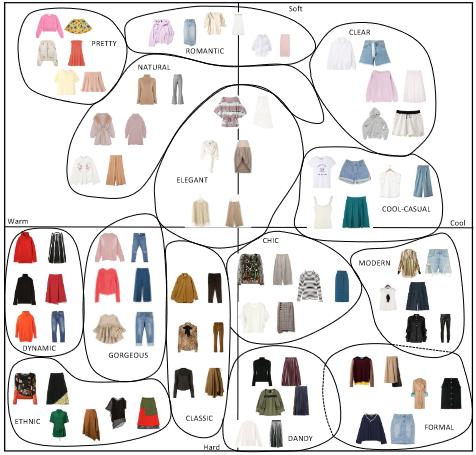
\includegraphics{img/styles}
	\caption{Label per la raccomandazione in Style Based Outfit Recommendation} \label{figura:stili} 
\end{figure}

\subsection{Segmentatore}

Per quanto riguarda la presentazione delle immagini degli indumenti è stato necessario l'uso di un segmentatore. Questo perchè altrimenti le foto sarebbero state salvate così come erano, introducendo non pochi problemi come:
\begin{itemize}
\item Estetica: lasciare nell'immagine ulteriori oggetti esterni fuori del contesto dell'indumento sarebbe stato in prima parte poco gradevole dal punto di vista visivo. 
\item Usabilità: l'eliminazione di soggetti estranei rende più intuibile che l'immagine riportata rappresenta totalmente un indumento, impedendo in questo modo incomprensioni da parte dell'utente.
\item Correttezza: la presenza di corpi estranei avrebbe potuto influenzare negativamente l'azione dei modelli che forniscono gli abbinamenti. Ad esempio, il colore dei non indumenti avrebbe potuto influire sul colore totale dell'immagine, andando così a porre in background il vero colore di interesse, ovvero quello del vestito.
\end{itemize}

In particolare, la segmentazione di un'immagine nell'elaborazione digitale delle immagini è il processo di partizione di un'immagine in regioni significative. Viene utilizzata per ottenere una rappresentazione più compatta, per estrarre degli oggetti o come strumento per l'analisi delle immagini e permette di partizionare le immagini digitali in insiemi di pixel. Lo scopo della segmentazione è semplificare e/o cambiare la rappresentazione delle immagini in qualcosa che è più significativo e facile da analizzare.

La segmentazione è di solito utilizzata per localizzare oggetti e bordi (linee, curve, ecc.). Più precisamente, la segmentazione è il processo con il quale si classificano i pixel dell'immagine che hanno caratteristiche comuni, pertanto ciascun pixel in una regione è simile agli altri della stessa regione per una qualche proprietà o caratteristica (colore, intensità o texture). Regioni adiacenti sono significativamente differenti rispetto ad almeno una di queste caratteristiche. Il risultato di un'immagine segmentata è un insieme di segmenti che, collettivamente, coprono l'intera immagine. Nel nostro caso la segmentazione è stata utilizzata al fine di trovare i bordi dell'indumento, soggetto principale della foto, e successivamente ritagliarlo dallo sfondo.

In particolare abbiamo utilizzato Detectron2 un software proprietario di FaceBook AI Research,che implementa algoritmi di object-detection che hanno ormai raggiunto lo stato dell'arte. Ai fini del progetto è stata utilizzata la funzione di object-detection per identificare il vestito (che dovrebbe ricoprire la parte preponderante della foto) e i metodi per la instance segmentation in modo da ottenere la precisa squadratura dell'oggetto stesso.

Dal punto di vista prestazionale, il risultato, dopo aver fornito l'immagine di input, viene restituito mediamente dopo pochi secondi dal modello già addestrato. Sebbene le tempistiche potrebbero sembrare larghe, in realtà per il task prefissato rispecchiano le medie temporali di altri segmentatori in commercio. Per ovviare comunque al problema di dover far attendere l'utente sul risultato in uscita dalla rete è stato provveduto un sistema di caricamento che fornisce un feedback visivo sullo stato di avanzamento dell'operazione.

A livello tecnico, l'immagine acquisita dalle API che gestiscono la fotocamera viene codificata in base64 per essere inviata al server, dove viene processata dal segmentatore che prima la riconverte in png, la elabora, per poi ritornarla al front end al fine di essere memorizzata in locale, ovviamente in caso di azione di salvataggio.

\section{Base64}

Per quanto riguarda la memorizzazione in locale e il recupero delle immagini, abbiamo avuto la necessità di doverci affidare a un sistema di codifica facile e veloce, in modo da garantire sempre elevate prestazioni e una reattività tale da consentire agli utenti prontezza d'uso dell'applicativo. Abbiamo deciso di fare affidamento in questo caso al protocollo di codifica Base64, che ha rispettato tutte le richieste implementative e prestazionali del nostro progetto.

Andando nello specifico, Base64 è un gruppo di schemi di codifica da binario a testo che rappresentano dati binari (più specificamente, una sequenza di byte a 8 bit) in un formato stringa ASCII traducendo i dati in una rappresentazione radix -64. Ogni cifra Base64 non finale rappresenta esattamente 6 bit di dati. Tre byte a 8 bit (cioè un totale di 24 bit) possono quindi essere rappresentati da quattro cifre Base64 a 6 bit.

Comune a tutti gli schemi di codifica da binario a testo, Base64 è progettato per trasportare dati archiviati in formati binari attraverso canali che supportano in modo affidabile solo contenuto di testo. Base64 è particolarmente diffuso nel Web, dove i suoi usi includono la possibilità di incorporare file di immagine o altre risorse binarie all'interno di risorse testuali come file HTML e CSS , come nel caso del nostro progetto.

\section{HTTP}

In questa trattazione non possiamo non parlare del protocollo di comunicazione e trasferimento che ci ha permesso di far interagire il front end ed il back end dell'applicativo sviluppato. Questo perchè, al fine di inviare le immagini al server per essere processate dal segmentatore o dalle reti neurali oppure per riportarle elaborate nel backend, avevamo bisogno di un protocollo facile, veloce e sicuro che stabilisse una connessione comunicativa tra i due endpoint.

Nel dettaglio HTTP, o HyperText Transfer Protocol è un protocollo del livello applicativo che, come anticipato sopra, riesce a trasmettere informazioni sia sul web che in applicazioni, con la tipica architettura client-server. Le richieste al server HTTP vengono effettuate sulla porta 80 per mezzo del protocollo TCP, o Transmission Control Protocol, a livello di trasporto.

HTTP è  un protocollo che funziona con un'architettura di tipo client-server: il client effettua una richiesta  e il server la risposta inviata da un altro host.  Nell'uso corrente,  il client corrisponde al browser e il server alla macchina su cui risiede il sito  Esistono  quindi due tipi di messaggi HTTP: messaggi di richiesta e messaggi di risposta. 

In particolare ai fini del progetto abbiamo fatto uso delle richieste POST al fine di inviare il file in base64 al server per l'elaborazione logica, mentre una richiesta GET è stata sfruttata per riprendere i dati una volta finito il processo.

\section{JSON}

JSON è un formato perfetto per lo scambio di dati fra applicazioni client/server. In particolare nel nostro progetto è stato sfruttato per codificare le informazioni da memorizzare in locale e che rappresentano gli indumenti con la relativa foto e metadati necessari affinchè questa sia processata. 
I metodi JSON che abbiamo adoperato si integrano perfettamente con il metodo di codifica delle foto catturate dall'app, ovvero in base64, fornendo addirittura un campo specifico per questo tipo di dati.

\section{Flask}

Per quanto riguarda la gestione del back end, la scelta che abbiamo fatto è stata quella di affideraci a flask. Avevamo infatti bisogno di un framework completo in python che ci permettesse di ricevere richieste dal front end in modo da gestire le chiamate agli script in Python delle reti neurali che abbiamo utilizzato.

nel dettaglio Flask è quello che possiamo definire micro-framework, dato che non ha un nucleo complesso ma può essere esteso tramite numerosi plugin ed estensioni, che espone la possibilità di mantenere un server ed un debugger, fondamentali per poter far interagire l'utente della web app con il codice delle reti neurali.

Abbiamo sfruttato la sua funzionalità di server in modo da poter ricevere ed inviare dati al front end tramite delle chiamate a richieste HTTP. I dati ricevuti, chiaramente, vengono dati in input ai vari modelli per la categorizzazione e la segmentazione che li processano e li restituiscono come output da reinviare al client.





% \include{files/chapter2}
\chapter{Conclusioni}\label{ch:conclusioni}
\ldots

\addcontentsline{toc}{chapter}{Bibliografia}
\bibliographystyle{plain}
\bibliography{files/biblio}
\bibliographystyle{unsrt}
%\bibliography{sp,xml}

\end{document} 